\documentclass[11pt]{article}

    \usepackage[breakable]{tcolorbox}
    \usepackage{parskip} % Stop auto-indenting (to mimic markdown behaviour)
    

    % Basic figure setup, for now with no caption control since it's done
    % automatically by Pandoc (which extracts ![](path) syntax from Markdown).
    \usepackage{graphicx}
    % Maintain compatibility with old templates. Remove in nbconvert 6.0
    \let\Oldincludegraphics\includegraphics
    % Ensure that by default, figures have no caption (until we provide a
    % proper Figure object with a Caption API and a way to capture that
    % in the conversion process - todo).
    \usepackage{caption}
    \DeclareCaptionFormat{nocaption}{}
    \captionsetup{format=nocaption,aboveskip=0pt,belowskip=0pt}

    \usepackage{float}
    \floatplacement{figure}{H} % forces figures to be placed at the correct location
    \usepackage{xcolor} % Allow colors to be defined
    \usepackage{enumerate} % Needed for markdown enumerations to work
    \usepackage{geometry} % Used to adjust the document margins
    \usepackage{amsmath} % Equations
    \usepackage{amssymb} % Equations
    \usepackage{textcomp} % defines textquotesingle
    % Hack from http://tex.stackexchange.com/a/47451/13684:
    \AtBeginDocument{%
        \def\PYZsq{\textquotesingle}% Upright quotes in Pygmentized code
    }
    \usepackage{upquote} % Upright quotes for verbatim code
    \usepackage{eurosym} % defines \euro

    \usepackage{iftex}
    \ifPDFTeX
        \usepackage[T1]{fontenc}
        \IfFileExists{alphabeta.sty}{
              \usepackage{alphabeta}
          }{
              \usepackage[mathletters]{ucs}
              \usepackage[utf8x]{inputenc}
          }
    \else
        \usepackage{fontspec}
        \usepackage{unicode-math}
    \fi

    \usepackage{fancyvrb} % verbatim replacement that allows latex
    \usepackage{grffile} % extends the file name processing of package graphics 
                         % to support a larger range
    \makeatletter % fix for old versions of grffile with XeLaTeX
    \@ifpackagelater{grffile}{2019/11/01}
    {
      % Do nothing on new versions
    }
    {
      \def\Gread@@xetex#1{%
        \IfFileExists{"\Gin@base".bb}%
        {\Gread@eps{\Gin@base.bb}}%
        {\Gread@@xetex@aux#1}%
      }
    }
    \makeatother
    \usepackage[Export]{adjustbox} % Used to constrain images to a maximum size
    \adjustboxset{max size={0.9\linewidth}{0.9\paperheight}}

    % The hyperref package gives us a pdf with properly built
    % internal navigation ('pdf bookmarks' for the table of contents,
    % internal cross-reference links, web links for URLs, etc.)
    \usepackage{hyperref}
    % The default LaTeX title has an obnoxious amount of whitespace. By default,
    % titling removes some of it. It also provides customization options.
    \usepackage{titling}
    \usepackage{longtable} % longtable support required by pandoc >1.10
    \usepackage{booktabs}  % table support for pandoc > 1.12.2
    \usepackage{array}     % table support for pandoc >= 2.11.3
    \usepackage{calc}      % table minipage width calculation for pandoc >= 2.11.1
    \usepackage[inline]{enumitem} % IRkernel/repr support (it uses the enumerate* environment)
    \usepackage[normalem]{ulem} % ulem is needed to support strikethroughs (\sout)
                                % normalem makes italics be italics, not underlines
    \usepackage{mathrsfs}
    

    
    % Colors for the hyperref package
    \definecolor{urlcolor}{rgb}{0,.145,.698}
    \definecolor{linkcolor}{rgb}{.71,0.21,0.01}
    \definecolor{citecolor}{rgb}{.12,.54,.11}

    % ANSI colors
    \definecolor{ansi-black}{HTML}{3E424D}
    \definecolor{ansi-black-intense}{HTML}{282C36}
    \definecolor{ansi-red}{HTML}{E75C58}
    \definecolor{ansi-red-intense}{HTML}{B22B31}
    \definecolor{ansi-green}{HTML}{00A250}
    \definecolor{ansi-green-intense}{HTML}{007427}
    \definecolor{ansi-yellow}{HTML}{DDB62B}
    \definecolor{ansi-yellow-intense}{HTML}{B27D12}
    \definecolor{ansi-blue}{HTML}{208FFB}
    \definecolor{ansi-blue-intense}{HTML}{0065CA}
    \definecolor{ansi-magenta}{HTML}{D160C4}
    \definecolor{ansi-magenta-intense}{HTML}{A03196}
    \definecolor{ansi-cyan}{HTML}{60C6C8}
    \definecolor{ansi-cyan-intense}{HTML}{258F8F}
    \definecolor{ansi-white}{HTML}{C5C1B4}
    \definecolor{ansi-white-intense}{HTML}{A1A6B2}
    \definecolor{ansi-default-inverse-fg}{HTML}{FFFFFF}
    \definecolor{ansi-default-inverse-bg}{HTML}{000000}

    % common color for the border for error outputs.
    \definecolor{outerrorbackground}{HTML}{FFDFDF}

    % commands and environments needed by pandoc snippets
    % extracted from the output of `pandoc -s`
    \providecommand{\tightlist}{%
      \setlength{\itemsep}{0pt}\setlength{\parskip}{0pt}}
    \DefineVerbatimEnvironment{Highlighting}{Verbatim}{commandchars=\\\{\}}
    % Add ',fontsize=\small' for more characters per line
    \newenvironment{Shaded}{}{}
    \newcommand{\KeywordTok}[1]{\textcolor[rgb]{0.00,0.44,0.13}{\textbf{{#1}}}}
    \newcommand{\DataTypeTok}[1]{\textcolor[rgb]{0.56,0.13,0.00}{{#1}}}
    \newcommand{\DecValTok}[1]{\textcolor[rgb]{0.25,0.63,0.44}{{#1}}}
    \newcommand{\BaseNTok}[1]{\textcolor[rgb]{0.25,0.63,0.44}{{#1}}}
    \newcommand{\FloatTok}[1]{\textcolor[rgb]{0.25,0.63,0.44}{{#1}}}
    \newcommand{\CharTok}[1]{\textcolor[rgb]{0.25,0.44,0.63}{{#1}}}
    \newcommand{\StringTok}[1]{\textcolor[rgb]{0.25,0.44,0.63}{{#1}}}
    \newcommand{\CommentTok}[1]{\textcolor[rgb]{0.38,0.63,0.69}{\textit{{#1}}}}
    \newcommand{\OtherTok}[1]{\textcolor[rgb]{0.00,0.44,0.13}{{#1}}}
    \newcommand{\AlertTok}[1]{\textcolor[rgb]{1.00,0.00,0.00}{\textbf{{#1}}}}
    \newcommand{\FunctionTok}[1]{\textcolor[rgb]{0.02,0.16,0.49}{{#1}}}
    \newcommand{\RegionMarkerTok}[1]{{#1}}
    \newcommand{\ErrorTok}[1]{\textcolor[rgb]{1.00,0.00,0.00}{\textbf{{#1}}}}
    \newcommand{\NormalTok}[1]{{#1}}
    
    % Additional commands for more recent versions of Pandoc
    \newcommand{\ConstantTok}[1]{\textcolor[rgb]{0.53,0.00,0.00}{{#1}}}
    \newcommand{\SpecialCharTok}[1]{\textcolor[rgb]{0.25,0.44,0.63}{{#1}}}
    \newcommand{\VerbatimStringTok}[1]{\textcolor[rgb]{0.25,0.44,0.63}{{#1}}}
    \newcommand{\SpecialStringTok}[1]{\textcolor[rgb]{0.73,0.40,0.53}{{#1}}}
    \newcommand{\ImportTok}[1]{{#1}}
    \newcommand{\DocumentationTok}[1]{\textcolor[rgb]{0.73,0.13,0.13}{\textit{{#1}}}}
    \newcommand{\AnnotationTok}[1]{\textcolor[rgb]{0.38,0.63,0.69}{\textbf{\textit{{#1}}}}}
    \newcommand{\CommentVarTok}[1]{\textcolor[rgb]{0.38,0.63,0.69}{\textbf{\textit{{#1}}}}}
    \newcommand{\VariableTok}[1]{\textcolor[rgb]{0.10,0.09,0.49}{{#1}}}
    \newcommand{\ControlFlowTok}[1]{\textcolor[rgb]{0.00,0.44,0.13}{\textbf{{#1}}}}
    \newcommand{\OperatorTok}[1]{\textcolor[rgb]{0.40,0.40,0.40}{{#1}}}
    \newcommand{\BuiltInTok}[1]{{#1}}
    \newcommand{\ExtensionTok}[1]{{#1}}
    \newcommand{\PreprocessorTok}[1]{\textcolor[rgb]{0.74,0.48,0.00}{{#1}}}
    \newcommand{\AttributeTok}[1]{\textcolor[rgb]{0.49,0.56,0.16}{{#1}}}
    \newcommand{\InformationTok}[1]{\textcolor[rgb]{0.38,0.63,0.69}{\textbf{\textit{{#1}}}}}
    \newcommand{\WarningTok}[1]{\textcolor[rgb]{0.38,0.63,0.69}{\textbf{\textit{{#1}}}}}
    
    
    % Define a nice break command that doesn't care if a line doesn't already
    % exist.
    \def\br{\hspace*{\fill} \\* }
    % Math Jax compatibility definitions
    \def\gt{>}
    \def\lt{<}
    \let\Oldtex\TeX
    \let\Oldlatex\LaTeX
    \renewcommand{\TeX}{\textrm{\Oldtex}}
    \renewcommand{\LaTeX}{\textrm{\Oldlatex}}
    % Document parameters
    % Document title
    \title{Lab04}
    
    
    
    
    
% Pygments definitions
\makeatletter
\def\PY@reset{\let\PY@it=\relax \let\PY@bf=\relax%
    \let\PY@ul=\relax \let\PY@tc=\relax%
    \let\PY@bc=\relax \let\PY@ff=\relax}
\def\PY@tok#1{\csname PY@tok@#1\endcsname}
\def\PY@toks#1+{\ifx\relax#1\empty\else%
    \PY@tok{#1}\expandafter\PY@toks\fi}
\def\PY@do#1{\PY@bc{\PY@tc{\PY@ul{%
    \PY@it{\PY@bf{\PY@ff{#1}}}}}}}
\def\PY#1#2{\PY@reset\PY@toks#1+\relax+\PY@do{#2}}

\@namedef{PY@tok@w}{\def\PY@tc##1{\textcolor[rgb]{0.73,0.73,0.73}{##1}}}
\@namedef{PY@tok@c}{\let\PY@it=\textit\def\PY@tc##1{\textcolor[rgb]{0.24,0.48,0.48}{##1}}}
\@namedef{PY@tok@cp}{\def\PY@tc##1{\textcolor[rgb]{0.61,0.40,0.00}{##1}}}
\@namedef{PY@tok@k}{\let\PY@bf=\textbf\def\PY@tc##1{\textcolor[rgb]{0.00,0.50,0.00}{##1}}}
\@namedef{PY@tok@kp}{\def\PY@tc##1{\textcolor[rgb]{0.00,0.50,0.00}{##1}}}
\@namedef{PY@tok@kt}{\def\PY@tc##1{\textcolor[rgb]{0.69,0.00,0.25}{##1}}}
\@namedef{PY@tok@o}{\def\PY@tc##1{\textcolor[rgb]{0.40,0.40,0.40}{##1}}}
\@namedef{PY@tok@ow}{\let\PY@bf=\textbf\def\PY@tc##1{\textcolor[rgb]{0.67,0.13,1.00}{##1}}}
\@namedef{PY@tok@nb}{\def\PY@tc##1{\textcolor[rgb]{0.00,0.50,0.00}{##1}}}
\@namedef{PY@tok@nf}{\def\PY@tc##1{\textcolor[rgb]{0.00,0.00,1.00}{##1}}}
\@namedef{PY@tok@nc}{\let\PY@bf=\textbf\def\PY@tc##1{\textcolor[rgb]{0.00,0.00,1.00}{##1}}}
\@namedef{PY@tok@nn}{\let\PY@bf=\textbf\def\PY@tc##1{\textcolor[rgb]{0.00,0.00,1.00}{##1}}}
\@namedef{PY@tok@ne}{\let\PY@bf=\textbf\def\PY@tc##1{\textcolor[rgb]{0.80,0.25,0.22}{##1}}}
\@namedef{PY@tok@nv}{\def\PY@tc##1{\textcolor[rgb]{0.10,0.09,0.49}{##1}}}
\@namedef{PY@tok@no}{\def\PY@tc##1{\textcolor[rgb]{0.53,0.00,0.00}{##1}}}
\@namedef{PY@tok@nl}{\def\PY@tc##1{\textcolor[rgb]{0.46,0.46,0.00}{##1}}}
\@namedef{PY@tok@ni}{\let\PY@bf=\textbf\def\PY@tc##1{\textcolor[rgb]{0.44,0.44,0.44}{##1}}}
\@namedef{PY@tok@na}{\def\PY@tc##1{\textcolor[rgb]{0.41,0.47,0.13}{##1}}}
\@namedef{PY@tok@nt}{\let\PY@bf=\textbf\def\PY@tc##1{\textcolor[rgb]{0.00,0.50,0.00}{##1}}}
\@namedef{PY@tok@nd}{\def\PY@tc##1{\textcolor[rgb]{0.67,0.13,1.00}{##1}}}
\@namedef{PY@tok@s}{\def\PY@tc##1{\textcolor[rgb]{0.73,0.13,0.13}{##1}}}
\@namedef{PY@tok@sd}{\let\PY@it=\textit\def\PY@tc##1{\textcolor[rgb]{0.73,0.13,0.13}{##1}}}
\@namedef{PY@tok@si}{\let\PY@bf=\textbf\def\PY@tc##1{\textcolor[rgb]{0.64,0.35,0.47}{##1}}}
\@namedef{PY@tok@se}{\let\PY@bf=\textbf\def\PY@tc##1{\textcolor[rgb]{0.67,0.36,0.12}{##1}}}
\@namedef{PY@tok@sr}{\def\PY@tc##1{\textcolor[rgb]{0.64,0.35,0.47}{##1}}}
\@namedef{PY@tok@ss}{\def\PY@tc##1{\textcolor[rgb]{0.10,0.09,0.49}{##1}}}
\@namedef{PY@tok@sx}{\def\PY@tc##1{\textcolor[rgb]{0.00,0.50,0.00}{##1}}}
\@namedef{PY@tok@m}{\def\PY@tc##1{\textcolor[rgb]{0.40,0.40,0.40}{##1}}}
\@namedef{PY@tok@gh}{\let\PY@bf=\textbf\def\PY@tc##1{\textcolor[rgb]{0.00,0.00,0.50}{##1}}}
\@namedef{PY@tok@gu}{\let\PY@bf=\textbf\def\PY@tc##1{\textcolor[rgb]{0.50,0.00,0.50}{##1}}}
\@namedef{PY@tok@gd}{\def\PY@tc##1{\textcolor[rgb]{0.63,0.00,0.00}{##1}}}
\@namedef{PY@tok@gi}{\def\PY@tc##1{\textcolor[rgb]{0.00,0.52,0.00}{##1}}}
\@namedef{PY@tok@gr}{\def\PY@tc##1{\textcolor[rgb]{0.89,0.00,0.00}{##1}}}
\@namedef{PY@tok@ge}{\let\PY@it=\textit}
\@namedef{PY@tok@gs}{\let\PY@bf=\textbf}
\@namedef{PY@tok@ges}{\let\PY@bf=\textbf\let\PY@it=\textit}
\@namedef{PY@tok@gp}{\let\PY@bf=\textbf\def\PY@tc##1{\textcolor[rgb]{0.00,0.00,0.50}{##1}}}
\@namedef{PY@tok@go}{\def\PY@tc##1{\textcolor[rgb]{0.44,0.44,0.44}{##1}}}
\@namedef{PY@tok@gt}{\def\PY@tc##1{\textcolor[rgb]{0.00,0.27,0.87}{##1}}}
\@namedef{PY@tok@err}{\def\PY@bc##1{{\setlength{\fboxsep}{\string -\fboxrule}\fcolorbox[rgb]{1.00,0.00,0.00}{1,1,1}{\strut ##1}}}}
\@namedef{PY@tok@kc}{\let\PY@bf=\textbf\def\PY@tc##1{\textcolor[rgb]{0.00,0.50,0.00}{##1}}}
\@namedef{PY@tok@kd}{\let\PY@bf=\textbf\def\PY@tc##1{\textcolor[rgb]{0.00,0.50,0.00}{##1}}}
\@namedef{PY@tok@kn}{\let\PY@bf=\textbf\def\PY@tc##1{\textcolor[rgb]{0.00,0.50,0.00}{##1}}}
\@namedef{PY@tok@kr}{\let\PY@bf=\textbf\def\PY@tc##1{\textcolor[rgb]{0.00,0.50,0.00}{##1}}}
\@namedef{PY@tok@bp}{\def\PY@tc##1{\textcolor[rgb]{0.00,0.50,0.00}{##1}}}
\@namedef{PY@tok@fm}{\def\PY@tc##1{\textcolor[rgb]{0.00,0.00,1.00}{##1}}}
\@namedef{PY@tok@vc}{\def\PY@tc##1{\textcolor[rgb]{0.10,0.09,0.49}{##1}}}
\@namedef{PY@tok@vg}{\def\PY@tc##1{\textcolor[rgb]{0.10,0.09,0.49}{##1}}}
\@namedef{PY@tok@vi}{\def\PY@tc##1{\textcolor[rgb]{0.10,0.09,0.49}{##1}}}
\@namedef{PY@tok@vm}{\def\PY@tc##1{\textcolor[rgb]{0.10,0.09,0.49}{##1}}}
\@namedef{PY@tok@sa}{\def\PY@tc##1{\textcolor[rgb]{0.73,0.13,0.13}{##1}}}
\@namedef{PY@tok@sb}{\def\PY@tc##1{\textcolor[rgb]{0.73,0.13,0.13}{##1}}}
\@namedef{PY@tok@sc}{\def\PY@tc##1{\textcolor[rgb]{0.73,0.13,0.13}{##1}}}
\@namedef{PY@tok@dl}{\def\PY@tc##1{\textcolor[rgb]{0.73,0.13,0.13}{##1}}}
\@namedef{PY@tok@s2}{\def\PY@tc##1{\textcolor[rgb]{0.73,0.13,0.13}{##1}}}
\@namedef{PY@tok@sh}{\def\PY@tc##1{\textcolor[rgb]{0.73,0.13,0.13}{##1}}}
\@namedef{PY@tok@s1}{\def\PY@tc##1{\textcolor[rgb]{0.73,0.13,0.13}{##1}}}
\@namedef{PY@tok@mb}{\def\PY@tc##1{\textcolor[rgb]{0.40,0.40,0.40}{##1}}}
\@namedef{PY@tok@mf}{\def\PY@tc##1{\textcolor[rgb]{0.40,0.40,0.40}{##1}}}
\@namedef{PY@tok@mh}{\def\PY@tc##1{\textcolor[rgb]{0.40,0.40,0.40}{##1}}}
\@namedef{PY@tok@mi}{\def\PY@tc##1{\textcolor[rgb]{0.40,0.40,0.40}{##1}}}
\@namedef{PY@tok@il}{\def\PY@tc##1{\textcolor[rgb]{0.40,0.40,0.40}{##1}}}
\@namedef{PY@tok@mo}{\def\PY@tc##1{\textcolor[rgb]{0.40,0.40,0.40}{##1}}}
\@namedef{PY@tok@ch}{\let\PY@it=\textit\def\PY@tc##1{\textcolor[rgb]{0.24,0.48,0.48}{##1}}}
\@namedef{PY@tok@cm}{\let\PY@it=\textit\def\PY@tc##1{\textcolor[rgb]{0.24,0.48,0.48}{##1}}}
\@namedef{PY@tok@cpf}{\let\PY@it=\textit\def\PY@tc##1{\textcolor[rgb]{0.24,0.48,0.48}{##1}}}
\@namedef{PY@tok@c1}{\let\PY@it=\textit\def\PY@tc##1{\textcolor[rgb]{0.24,0.48,0.48}{##1}}}
\@namedef{PY@tok@cs}{\let\PY@it=\textit\def\PY@tc##1{\textcolor[rgb]{0.24,0.48,0.48}{##1}}}

\def\PYZbs{\char`\\}
\def\PYZus{\char`\_}
\def\PYZob{\char`\{}
\def\PYZcb{\char`\}}
\def\PYZca{\char`\^}
\def\PYZam{\char`\&}
\def\PYZlt{\char`\<}
\def\PYZgt{\char`\>}
\def\PYZsh{\char`\#}
\def\PYZpc{\char`\%}
\def\PYZdl{\char`\$}
\def\PYZhy{\char`\-}
\def\PYZsq{\char`\'}
\def\PYZdq{\char`\"}
\def\PYZti{\char`\~}
% for compatibility with earlier versions
\def\PYZat{@}
\def\PYZlb{[}
\def\PYZrb{]}
\makeatother


    % For linebreaks inside Verbatim environment from package fancyvrb. 
    \makeatletter
        \newbox\Wrappedcontinuationbox 
        \newbox\Wrappedvisiblespacebox 
        \newcommand*\Wrappedvisiblespace {\textcolor{red}{\textvisiblespace}} 
        \newcommand*\Wrappedcontinuationsymbol {\textcolor{red}{\llap{\tiny$\m@th\hookrightarrow$}}} 
        \newcommand*\Wrappedcontinuationindent {3ex } 
        \newcommand*\Wrappedafterbreak {\kern\Wrappedcontinuationindent\copy\Wrappedcontinuationbox} 
        % Take advantage of the already applied Pygments mark-up to insert 
        % potential linebreaks for TeX processing. 
        %        {, <, #, %, $, ' and ": go to next line. 
        %        _, }, ^, &, >, - and ~: stay at end of broken line. 
        % Use of \textquotesingle for straight quote. 
        \newcommand*\Wrappedbreaksatspecials {% 
            \def\PYGZus{\discretionary{\char`\_}{\Wrappedafterbreak}{\char`\_}}% 
            \def\PYGZob{\discretionary{}{\Wrappedafterbreak\char`\{}{\char`\{}}% 
            \def\PYGZcb{\discretionary{\char`\}}{\Wrappedafterbreak}{\char`\}}}% 
            \def\PYGZca{\discretionary{\char`\^}{\Wrappedafterbreak}{\char`\^}}% 
            \def\PYGZam{\discretionary{\char`\&}{\Wrappedafterbreak}{\char`\&}}% 
            \def\PYGZlt{\discretionary{}{\Wrappedafterbreak\char`\<}{\char`\<}}% 
            \def\PYGZgt{\discretionary{\char`\>}{\Wrappedafterbreak}{\char`\>}}% 
            \def\PYGZsh{\discretionary{}{\Wrappedafterbreak\char`\#}{\char`\#}}% 
            \def\PYGZpc{\discretionary{}{\Wrappedafterbreak\char`\%}{\char`\%}}% 
            \def\PYGZdl{\discretionary{}{\Wrappedafterbreak\char`\$}{\char`\$}}% 
            \def\PYGZhy{\discretionary{\char`\-}{\Wrappedafterbreak}{\char`\-}}% 
            \def\PYGZsq{\discretionary{}{\Wrappedafterbreak\textquotesingle}{\textquotesingle}}% 
            \def\PYGZdq{\discretionary{}{\Wrappedafterbreak\char`\"}{\char`\"}}% 
            \def\PYGZti{\discretionary{\char`\~}{\Wrappedafterbreak}{\char`\~}}% 
        } 
        % Some characters . , ; ? ! / are not pygmentized. 
        % This macro makes them "active" and they will insert potential linebreaks 
        \newcommand*\Wrappedbreaksatpunct {% 
            \lccode`\~`\.\lowercase{\def~}{\discretionary{\hbox{\char`\.}}{\Wrappedafterbreak}{\hbox{\char`\.}}}% 
            \lccode`\~`\,\lowercase{\def~}{\discretionary{\hbox{\char`\,}}{\Wrappedafterbreak}{\hbox{\char`\,}}}% 
            \lccode`\~`\;\lowercase{\def~}{\discretionary{\hbox{\char`\;}}{\Wrappedafterbreak}{\hbox{\char`\;}}}% 
            \lccode`\~`\:\lowercase{\def~}{\discretionary{\hbox{\char`\:}}{\Wrappedafterbreak}{\hbox{\char`\:}}}% 
            \lccode`\~`\?\lowercase{\def~}{\discretionary{\hbox{\char`\?}}{\Wrappedafterbreak}{\hbox{\char`\?}}}% 
            \lccode`\~`\!\lowercase{\def~}{\discretionary{\hbox{\char`\!}}{\Wrappedafterbreak}{\hbox{\char`\!}}}% 
            \lccode`\~`\/\lowercase{\def~}{\discretionary{\hbox{\char`\/}}{\Wrappedafterbreak}{\hbox{\char`\/}}}% 
            \catcode`\.\active
            \catcode`\,\active 
            \catcode`\;\active
            \catcode`\:\active
            \catcode`\?\active
            \catcode`\!\active
            \catcode`\/\active 
            \lccode`\~`\~ 	
        }
    \makeatother

    \let\OriginalVerbatim=\Verbatim
    \makeatletter
    \renewcommand{\Verbatim}[1][1]{%
        %\parskip\z@skip
        \sbox\Wrappedcontinuationbox {\Wrappedcontinuationsymbol}%
        \sbox\Wrappedvisiblespacebox {\FV@SetupFont\Wrappedvisiblespace}%
        \def\FancyVerbFormatLine ##1{\hsize\linewidth
            \vtop{\raggedright\hyphenpenalty\z@\exhyphenpenalty\z@
                \doublehyphendemerits\z@\finalhyphendemerits\z@
                \strut ##1\strut}%
        }%
        % If the linebreak is at a space, the latter will be displayed as visible
        % space at end of first line, and a continuation symbol starts next line.
        % Stretch/shrink are however usually zero for typewriter font.
        \def\FV@Space {%
            \nobreak\hskip\z@ plus\fontdimen3\font minus\fontdimen4\font
            \discretionary{\copy\Wrappedvisiblespacebox}{\Wrappedafterbreak}
            {\kern\fontdimen2\font}%
        }%
        
        % Allow breaks at special characters using \PYG... macros.
        \Wrappedbreaksatspecials
        % Breaks at punctuation characters . , ; ? ! and / need catcode=\active 	
        \OriginalVerbatim[#1,codes*=\Wrappedbreaksatpunct]%
    }
    \makeatother

    % Exact colors from NB
    \definecolor{incolor}{HTML}{303F9F}
    \definecolor{outcolor}{HTML}{D84315}
    \definecolor{cellborder}{HTML}{CFCFCF}
    \definecolor{cellbackground}{HTML}{F7F7F7}
    
    % prompt
    \makeatletter
    \newcommand{\boxspacing}{\kern\kvtcb@left@rule\kern\kvtcb@boxsep}
    \makeatother
    \newcommand{\prompt}[4]{
        {\ttfamily\llap{{\color{#2}[#3]:\hspace{3pt}#4}}\vspace{-\baselineskip}}
    }
    

    
    % Prevent overflowing lines due to hard-to-break entities
    \sloppy 
    % Setup hyperref package
    \hypersetup{
      breaklinks=true,  % so long urls are correctly broken across lines
      colorlinks=true,
      urlcolor=urlcolor,
      linkcolor=linkcolor,
      citecolor=citecolor,
      }
    % Slightly bigger margins than the latex defaults
    
    \geometry{verbose,tmargin=1in,bmargin=1in,lmargin=1in,rmargin=1in}
    
    

\begin{document}
    
    \maketitle
    
    

    
    \hypertarget{notebook}{%
\section{NOTEBOOK}\label{notebook}}

\hypertarget{parte-1---metriche-di-classificazione}{%
\section{PARTE 1 - METRICHE DI
CLASSIFICAZIONE}\label{parte-1---metriche-di-classificazione}}

\hypertarget{passo-1---setup-e-classificatore-serio}{%
\subsection{PASSO 1 - SETUP E CLASSIFICATORE
``SERIO''}\label{passo-1---setup-e-classificatore-serio}}

    \begin{tcolorbox}[breakable, size=fbox, boxrule=1pt, pad at break*=1mm,colback=cellbackground, colframe=cellborder]
\prompt{In}{incolor}{ }{\boxspacing}
\begin{Verbatim}[commandchars=\\\{\}]
\PY{k+kn}{from}\PY{+w}{ }\PY{n+nn}{sklearn}\PY{n+nn}{.}\PY{n+nn}{datasets}\PY{+w}{ }\PY{k+kn}{import} \PY{n}{fetch\PYZus{}openml}
\PY{k+kn}{from}\PY{+w}{ }\PY{n+nn}{sklearn}\PY{n+nn}{.}\PY{n+nn}{linear\PYZus{}model}\PY{+w}{ }\PY{k+kn}{import} \PY{n}{SGDClassifier}
\PY{k+kn}{from}\PY{+w}{ }\PY{n+nn}{sklearn}\PY{n+nn}{.}\PY{n+nn}{model\PYZus{}selection}\PY{+w}{ }\PY{k+kn}{import} \PY{n}{cross\PYZus{}val\PYZus{}predict}
\PY{k+kn}{from}\PY{+w}{ }\PY{n+nn}{sklearn}\PY{n+nn}{.}\PY{n+nn}{metrics}\PY{+w}{ }\PY{k+kn}{import} \PY{n}{confusion\PYZus{}matrix}\PY{p}{,} \PY{n}{precision\PYZus{}score}\PY{p}{,} \PY{n}{recall\PYZus{}score}\PY{p}{,} \PY{n}{f1\PYZus{}score}

\PY{c+c1}{\PYZsh{} 1. Caricamento MNIST}
\PY{n}{mnist} \PY{o}{=} \PY{n}{fetch\PYZus{}openml}\PY{p}{(}\PY{l+s+s2}{\PYZdq{}}\PY{l+s+s2}{mnist\PYZus{}784}\PY{l+s+s2}{\PYZdq{}}\PY{p}{,} \PY{n}{as\PYZus{}frame}\PY{o}{=}\PY{k+kc}{False}\PY{p}{,} \PY{n}{parser}\PY{o}{=}\PY{l+s+s1}{\PYZsq{}}\PY{l+s+s1}{auto}\PY{l+s+s1}{\PYZsq{}}\PY{p}{)}
\PY{n}{X}\PY{p}{,} \PY{n}{y} \PY{o}{=} \PY{n}{mnist}\PY{p}{[}\PY{l+s+s2}{\PYZdq{}}\PY{l+s+s2}{data}\PY{l+s+s2}{\PYZdq{}}\PY{p}{]}\PY{p}{,} \PY{n}{mnist}\PY{p}{[}\PY{l+s+s2}{\PYZdq{}}\PY{l+s+s2}{target}\PY{l+s+s2}{\PYZdq{}}\PY{p}{]}\PY{o}{.}\PY{n}{astype}\PY{p}{(}\PY{n+nb}{int}\PY{p}{)}

\PY{c+c1}{\PYZsh{} 2. Train/test split come da libro}
\PY{n}{X\PYZus{}train}\PY{p}{,} \PY{n}{X\PYZus{}test} \PY{o}{=} \PY{n}{X}\PY{p}{[}\PY{p}{:}\PY{l+m+mi}{60000}\PY{p}{]}\PY{p}{,} \PY{n}{X}\PY{p}{[}\PY{l+m+mi}{60000}\PY{p}{:}\PY{p}{]}
\PY{n}{y\PYZus{}train}\PY{p}{,} \PY{n}{y\PYZus{}test} \PY{o}{=} \PY{n}{y}\PY{p}{[}\PY{p}{:}\PY{l+m+mi}{60000}\PY{p}{]}\PY{p}{,} \PY{n}{y}\PY{p}{[}\PY{l+m+mi}{60000}\PY{p}{:}\PY{p}{]}

\PY{c+c1}{\PYZsh{} 3. Problema binario: 5 vs non\PYZhy{}5}
\PY{n}{y\PYZus{}train\PYZus{}5} \PY{o}{=} \PY{p}{(}\PY{n}{y\PYZus{}train} \PY{o}{==} \PY{l+m+mi}{5}\PY{p}{)}
\PY{n}{y\PYZus{}test\PYZus{}5} \PY{o}{=} \PY{p}{(}\PY{n}{y\PYZus{}test} \PY{o}{==} \PY{l+m+mi}{5}\PY{p}{)}

\PY{c+c1}{\PYZsh{} 4. Classificatore lineare}
\PY{n}{sgd\PYZus{}clf} \PY{o}{=} \PY{n}{SGDClassifier}\PY{p}{(}\PY{n}{random\PYZus{}state}\PY{o}{=}\PY{l+m+mi}{42}\PY{p}{)}
\PY{n}{y\PYZus{}train\PYZus{}pred} \PY{o}{=} \PY{n}{cross\PYZus{}val\PYZus{}predict}\PY{p}{(}\PY{n}{sgd\PYZus{}clf}\PY{p}{,} \PY{n}{X\PYZus{}train}\PY{p}{,} \PY{n}{y\PYZus{}train\PYZus{}5}\PY{p}{,} \PY{n}{cv}\PY{o}{=}\PY{l+m+mi}{3}\PY{p}{)}
\end{Verbatim}
\end{tcolorbox}

    \hypertarget{matrice-di-confusione}{%
\subsubsection{Matrice di confusione}\label{matrice-di-confusione}}

    \begin{tcolorbox}[breakable, size=fbox, boxrule=1pt, pad at break*=1mm,colback=cellbackground, colframe=cellborder]
\prompt{In}{incolor}{ }{\boxspacing}
\begin{Verbatim}[commandchars=\\\{\}]
\PY{n}{cm} \PY{o}{=} \PY{n}{confusion\PYZus{}matrix}\PY{p}{(}\PY{n}{y\PYZus{}train\PYZus{}5}\PY{p}{,} \PY{n}{y\PYZus{}train\PYZus{}pred}\PY{p}{)}
\PY{n+nb}{print}\PY{p}{(}\PY{n}{cm}\PY{p}{)}
\end{Verbatim}
\end{tcolorbox}

    \hypertarget{identificazione-tn-fp-fn-tp}{%
\subsubsection{Identificazione TN, FP, FN,
TP}\label{identificazione-tn-fp-fn-tp}}

    \begin{tcolorbox}[breakable, size=fbox, boxrule=1pt, pad at break*=1mm,colback=cellbackground, colframe=cellborder]
\prompt{In}{incolor}{ }{\boxspacing}
\begin{Verbatim}[commandchars=\\\{\}]
\PY{n}{TN} \PY{o}{=} \PY{n}{cm}\PY{p}{[}\PY{l+m+mi}{0}\PY{p}{,}\PY{l+m+mi}{0}\PY{p}{]}
\PY{n}{FP} \PY{o}{=} \PY{n}{cm}\PY{p}{[}\PY{l+m+mi}{0}\PY{p}{,}\PY{l+m+mi}{1}\PY{p}{]}
\PY{n}{FN} \PY{o}{=} \PY{n}{cm}\PY{p}{[}\PY{l+m+mi}{1}\PY{p}{,}\PY{l+m+mi}{0}\PY{p}{]}
\PY{n}{TP} \PY{o}{=} \PY{n}{cm}\PY{p}{[}\PY{l+m+mi}{1}\PY{p}{,}\PY{l+m+mi}{1}\PY{p}{]}
\end{Verbatim}
\end{tcolorbox}

    \hypertarget{calcolo-di-precision-recall-f1-e-accuracy}{%
\subsubsection{Calcolo di Precision, Recall, F1 e
Accuracy}\label{calcolo-di-precision-recall-f1-e-accuracy}}

    \begin{tcolorbox}[breakable, size=fbox, boxrule=1pt, pad at break*=1mm,colback=cellbackground, colframe=cellborder]
\prompt{In}{incolor}{ }{\boxspacing}
\begin{Verbatim}[commandchars=\\\{\}]
\PY{n}{precision} \PY{o}{=} \PY{n}{TP} \PY{o}{/} \PY{p}{(}\PY{n}{TP} \PY{o}{+} \PY{n}{FP}\PY{p}{)}
\PY{n}{recall} \PY{o}{=} \PY{n}{TP} \PY{o}{/} \PY{p}{(}\PY{n}{TP} \PY{o}{+} \PY{n}{FN}\PY{p}{)}
\PY{n}{f1} \PY{o}{=} \PY{l+m+mi}{2} \PY{o}{*} \PY{n}{precision} \PY{o}{*} \PY{n}{recall} \PY{o}{/} \PY{p}{(}\PY{n}{precision} \PY{o}{+} \PY{n}{recall}\PY{p}{)}

\PY{n+nb}{print}\PY{p}{(}\PY{l+s+sa}{f}\PY{l+s+s2}{\PYZdq{}}\PY{l+s+s2}{Precision Score: }\PY{l+s+si}{\PYZob{}}\PY{n}{precision}\PY{l+s+si}{:}\PY{l+s+s2}{.2f}\PY{l+s+si}{\PYZcb{}}\PY{l+s+s2}{\PYZdq{}}\PY{p}{)}
\PY{n+nb}{print}\PY{p}{(}\PY{l+s+sa}{f}\PY{l+s+s2}{\PYZdq{}}\PY{l+s+s2}{Recall Score: }\PY{l+s+si}{\PYZob{}}\PY{n}{recall}\PY{l+s+si}{:}\PY{l+s+s2}{.2f}\PY{l+s+si}{\PYZcb{}}\PY{l+s+s2}{\PYZdq{}}\PY{p}{)}
\PY{n+nb}{print}\PY{p}{(}\PY{l+s+sa}{f}\PY{l+s+s2}{\PYZdq{}}\PY{l+s+s2}{F1 Score: }\PY{l+s+si}{\PYZob{}}\PY{n}{f1}\PY{l+s+si}{:}\PY{l+s+s2}{.2f}\PY{l+s+si}{\PYZcb{}}\PY{l+s+s2}{\PYZdq{}}\PY{p}{)}
\end{Verbatim}
\end{tcolorbox}

    \hypertarget{passo-2---dummy-classifier-e-accuracy-ingannevole}{%
\subsection{PASSO 2 - DUMMY CLASSIFIER E ACCURACY
INGANNEVOLE}\label{passo-2---dummy-classifier-e-accuracy-ingannevole}}

    \begin{tcolorbox}[breakable, size=fbox, boxrule=1pt, pad at break*=1mm,colback=cellbackground, colframe=cellborder]
\prompt{In}{incolor}{ }{\boxspacing}
\begin{Verbatim}[commandchars=\\\{\}]
\PY{k+kn}{from}\PY{+w}{ }\PY{n+nn}{sklearn}\PY{n+nn}{.}\PY{n+nn}{base}\PY{+w}{ }\PY{k+kn}{import} \PY{n}{BaseEstimator}
\PY{k+kn}{from}\PY{+w}{ }\PY{n+nn}{sklearn}\PY{n+nn}{.}\PY{n+nn}{metrics}\PY{+w}{ }\PY{k+kn}{import} \PY{n}{accuracy\PYZus{}score}
\PY{k+kn}{import}\PY{+w}{ }\PY{n+nn}{numpy}\PY{+w}{ }\PY{k}{as}\PY{+w}{ }\PY{n+nn}{np}

\PY{k}{class}\PY{+w}{ }\PY{n+nc}{NeverFiveClassifier}\PY{p}{(}\PY{n}{BaseEstimator}\PY{p}{)}\PY{p}{:}
    \PY{k}{def}\PY{+w}{ }\PY{n+nf}{fit}\PY{p}{(}\PY{n+nb+bp}{self}\PY{p}{,} \PY{n}{X}\PY{p}{,} \PY{n}{y}\PY{o}{=}\PY{k+kc}{None}\PY{p}{)}\PY{p}{:}
        \PY{k}{return} \PY{n+nb+bp}{self}
    \PY{k}{def}\PY{+w}{ }\PY{n+nf}{predict}\PY{p}{(}\PY{n+nb+bp}{self}\PY{p}{,} \PY{n}{X}\PY{p}{)}\PY{p}{:}
        \PY{k}{return} \PY{n}{np}\PY{o}{.}\PY{n}{zeros}\PY{p}{(}\PY{p}{(}\PY{n+nb}{len}\PY{p}{(}\PY{n}{X}\PY{p}{)}\PY{p}{,}\PY{p}{)}\PY{p}{,} \PY{n}{dtype}\PY{o}{=}\PY{n+nb}{bool}\PY{p}{)}

\PY{n}{never\PYZus{}clf} \PY{o}{=} \PY{n}{NeverFiveClassifier}\PY{p}{(}\PY{p}{)}
\PY{n}{y\PYZus{}train\PYZus{}pred\PYZus{}dummy} \PY{o}{=} \PY{n}{cross\PYZus{}val\PYZus{}predict}\PY{p}{(}\PY{n}{never\PYZus{}clf}\PY{p}{,} \PY{n}{X\PYZus{}train}\PY{p}{,} \PY{n}{y\PYZus{}train\PYZus{}5}\PY{p}{,} \PY{n}{cv}\PY{o}{=}\PY{l+m+mi}{3}\PY{p}{)}
\end{Verbatim}
\end{tcolorbox}

    \hypertarget{matrice-di-confusione-e-metriche-del-dummy-classifier}{%
\subsubsection{Matrice di confusione e metriche del dummy
classifier}\label{matrice-di-confusione-e-metriche-del-dummy-classifier}}

    \begin{tcolorbox}[breakable, size=fbox, boxrule=1pt, pad at break*=1mm,colback=cellbackground, colframe=cellborder]
\prompt{In}{incolor}{ }{\boxspacing}
\begin{Verbatim}[commandchars=\\\{\}]
\PY{n}{cm\PYZus{}dummy} \PY{o}{=} \PY{n}{confusion\PYZus{}matrix}\PY{p}{(}\PY{n}{y\PYZus{}train\PYZus{}5}\PY{p}{,} \PY{n}{y\PYZus{}train\PYZus{}pred\PYZus{}dummy}\PY{p}{)}
\PY{n+nb}{print}\PY{p}{(}\PY{n}{cm\PYZus{}dummy}\PY{p}{)}

\PY{n}{TN\PYZus{}d} \PY{o}{=} \PY{n}{cm\PYZus{}dummy}\PY{p}{[}\PY{l+m+mi}{0}\PY{p}{,}\PY{l+m+mi}{0}\PY{p}{]}
\PY{n}{FP\PYZus{}d} \PY{o}{=} \PY{n}{cm\PYZus{}dummy}\PY{p}{[}\PY{l+m+mi}{0}\PY{p}{,}\PY{l+m+mi}{1}\PY{p}{]}
\PY{n}{FN\PYZus{}d} \PY{o}{=} \PY{n}{cm\PYZus{}dummy}\PY{p}{[}\PY{l+m+mi}{1}\PY{p}{,}\PY{l+m+mi}{0}\PY{p}{]}
\PY{n}{TP\PYZus{}d} \PY{o}{=} \PY{n}{cm\PYZus{}dummy}\PY{p}{[}\PY{l+m+mi}{1}\PY{p}{,}\PY{l+m+mi}{1}\PY{p}{]}

\PY{c+c1}{\PYZsh{} Accuracy}
\PY{n}{acc\PYZus{}dummy} \PY{o}{=} \PY{p}{(}\PY{n}{TP\PYZus{}d} \PY{o}{+} \PY{n}{TN\PYZus{}d}\PY{p}{)} \PY{o}{/} \PY{p}{(}\PY{n}{TP\PYZus{}d} \PY{o}{+} \PY{n}{TN\PYZus{}d} \PY{o}{+} \PY{n}{FP\PYZus{}d} \PY{o}{+} \PY{n}{FN\PYZus{}d}\PY{p}{)}
\PY{n+nb}{print}\PY{p}{(}\PY{l+s+sa}{f}\PY{l+s+s2}{\PYZdq{}}\PY{l+s+se}{\PYZbs{}n}\PY{l+s+s2}{Accuracy: }\PY{l+s+si}{\PYZob{}}\PY{n}{acc\PYZus{}dummy}\PY{l+s+si}{:}\PY{l+s+s2}{.3f}\PY{l+s+si}{\PYZcb{}}\PY{l+s+s2}{\PYZdq{}}\PY{p}{)}

\PY{n}{p\PYZus{}d} \PY{o}{=} \PY{n}{TP\PYZus{}d} \PY{o}{/} \PY{p}{(}\PY{n}{TP\PYZus{}d} \PY{o}{+} \PY{n}{FP\PYZus{}d}\PY{p}{)} \PY{k}{if} \PY{p}{(}\PY{n}{TP\PYZus{}d} \PY{o}{+} \PY{n}{FP\PYZus{}d}\PY{p}{)} \PY{o}{!=} \PY{l+m+mi}{0} \PY{k}{else} \PY{l+m+mf}{0.0}
\PY{n}{r\PYZus{}d} \PY{o}{=} \PY{n}{TP\PYZus{}d} \PY{o}{/} \PY{p}{(}\PY{n}{TP\PYZus{}d} \PY{o}{+} \PY{n}{FN\PYZus{}d}\PY{p}{)} \PY{k}{if} \PY{p}{(}\PY{n}{TP\PYZus{}d} \PY{o}{+} \PY{n}{FN\PYZus{}d}\PY{p}{)} \PY{o}{!=} \PY{l+m+mi}{0} \PY{k}{else} \PY{l+m+mf}{0.0}
\PY{n}{f1\PYZus{}d} \PY{o}{=} \PY{l+m+mi}{2} \PY{o}{*} \PY{n}{p\PYZus{}d} \PY{o}{*} \PY{n}{r\PYZus{}d} \PY{o}{/} \PY{p}{(}\PY{n}{p\PYZus{}d} \PY{o}{+} \PY{n}{r\PYZus{}d}\PY{p}{)} \PY{k}{if} \PY{p}{(}\PY{n}{p\PYZus{}d} \PY{o}{+} \PY{n}{r\PYZus{}d}\PY{p}{)} \PY{o}{!=} \PY{l+m+mi}{0} \PY{k}{else} \PY{l+m+mf}{0.0}

\PY{n+nb}{print}\PY{p}{(}\PY{l+s+sa}{f}\PY{l+s+s2}{\PYZdq{}}\PY{l+s+s2}{Precision Score: }\PY{l+s+si}{\PYZob{}}\PY{n}{p\PYZus{}d}\PY{l+s+si}{\PYZcb{}}\PY{l+s+s2}{\PYZdq{}}\PY{p}{)}
\PY{n+nb}{print}\PY{p}{(}\PY{l+s+sa}{f}\PY{l+s+s2}{\PYZdq{}}\PY{l+s+s2}{Recall Score: }\PY{l+s+si}{\PYZob{}}\PY{n}{r\PYZus{}d}\PY{l+s+si}{\PYZcb{}}\PY{l+s+s2}{\PYZdq{}}\PY{p}{)}
\PY{n+nb}{print}\PY{p}{(}\PY{l+s+sa}{f}\PY{l+s+s2}{\PYZdq{}}\PY{l+s+s2}{F1 Score: }\PY{l+s+si}{\PYZob{}}\PY{n}{f1\PYZus{}d}\PY{l+s+si}{\PYZcb{}}\PY{l+s+s2}{\PYZdq{}}\PY{p}{)}
\end{Verbatim}
\end{tcolorbox}

    \hypertarget{tabella-di-confronto}{%
\subsubsection{Tabella di confronto}\label{tabella-di-confronto}}

    \begin{tcolorbox}[breakable, size=fbox, boxrule=1pt, pad at break*=1mm,colback=cellbackground, colframe=cellborder]
\prompt{In}{incolor}{ }{\boxspacing}
\begin{Verbatim}[commandchars=\\\{\}]
\PY{k+kn}{import}\PY{+w}{ }\PY{n+nn}{pandas}\PY{+w}{ }\PY{k}{as}\PY{+w}{ }\PY{n+nn}{pd}

\PY{n}{confronto} \PY{o}{=} \PY{n}{pd}\PY{o}{.}\PY{n}{DataFrame}\PY{p}{(}\PY{p}{\PYZob{}}
    \PY{l+s+s2}{\PYZdq{}}\PY{l+s+s2}{Modello}\PY{l+s+s2}{\PYZdq{}}\PY{p}{:} \PY{p}{[}\PY{l+s+s2}{\PYZdq{}}\PY{l+s+s2}{SGD 5\PYZhy{}detector}\PY{l+s+s2}{\PYZdq{}}\PY{p}{,} \PY{l+s+s2}{\PYZdq{}}\PY{l+s+s2}{Never\PYZhy{}5}\PY{l+s+s2}{\PYZdq{}}\PY{p}{]}\PY{p}{,}
    \PY{l+s+s2}{\PYZdq{}}\PY{l+s+s2}{Accuracy}\PY{l+s+s2}{\PYZdq{}}\PY{p}{:} \PY{p}{[}\PY{l+s+sa}{f}\PY{l+s+s2}{\PYZdq{}}\PY{l+s+si}{\PYZob{}}\PY{n}{accuracy}\PY{l+s+si}{:}\PY{l+s+s2}{.2f}\PY{l+s+si}{\PYZcb{}}\PY{l+s+s2}{\PYZdq{}}\PY{p}{,} \PY{l+s+sa}{f}\PY{l+s+s2}{\PYZdq{}}\PY{l+s+si}{\PYZob{}}\PY{n}{acc\PYZus{}dummy}\PY{l+s+si}{:}\PY{l+s+s2}{.2f}\PY{l+s+si}{\PYZcb{}}\PY{l+s+s2}{\PYZdq{}}\PY{p}{]}\PY{p}{,}
    \PY{l+s+s2}{\PYZdq{}}\PY{l+s+s2}{Precision}\PY{l+s+s2}{\PYZdq{}}\PY{p}{:} \PY{p}{[}\PY{l+s+sa}{f}\PY{l+s+s2}{\PYZdq{}}\PY{l+s+si}{\PYZob{}}\PY{n}{precision}\PY{l+s+si}{:}\PY{l+s+s2}{.2f}\PY{l+s+si}{\PYZcb{}}\PY{l+s+s2}{\PYZdq{}}\PY{p}{,} \PY{l+s+sa}{f}\PY{l+s+s2}{\PYZdq{}}\PY{l+s+si}{\PYZob{}}\PY{n}{p\PYZus{}d}\PY{l+s+si}{:}\PY{l+s+s2}{.2f}\PY{l+s+si}{\PYZcb{}}\PY{l+s+s2}{\PYZdq{}}\PY{p}{]}\PY{p}{,}
    \PY{l+s+s2}{\PYZdq{}}\PY{l+s+s2}{Recall}\PY{l+s+s2}{\PYZdq{}}\PY{p}{:} \PY{p}{[}\PY{l+s+sa}{f}\PY{l+s+s2}{\PYZdq{}}\PY{l+s+si}{\PYZob{}}\PY{n}{recall}\PY{l+s+si}{:}\PY{l+s+s2}{.2f}\PY{l+s+si}{\PYZcb{}}\PY{l+s+s2}{\PYZdq{}}\PY{p}{,} \PY{l+s+sa}{f}\PY{l+s+s2}{\PYZdq{}}\PY{l+s+si}{\PYZob{}}\PY{n}{r\PYZus{}d}\PY{l+s+si}{:}\PY{l+s+s2}{.2f}\PY{l+s+si}{\PYZcb{}}\PY{l+s+s2}{\PYZdq{}}\PY{p}{]}\PY{p}{,}
    \PY{l+s+s2}{\PYZdq{}}\PY{l+s+s2}{F1}\PY{l+s+s2}{\PYZdq{}}\PY{p}{:} \PY{p}{[}\PY{l+s+sa}{f}\PY{l+s+s2}{\PYZdq{}}\PY{l+s+si}{\PYZob{}}\PY{n}{f1}\PY{l+s+si}{:}\PY{l+s+s2}{.2f}\PY{l+s+si}{\PYZcb{}}\PY{l+s+s2}{\PYZdq{}}\PY{p}{,} \PY{l+s+sa}{f}\PY{l+s+s2}{\PYZdq{}}\PY{l+s+si}{\PYZob{}}\PY{n}{f1\PYZus{}d}\PY{l+s+si}{:}\PY{l+s+s2}{.2f}\PY{l+s+si}{\PYZcb{}}\PY{l+s+s2}{\PYZdq{}}\PY{p}{]}
\PY{p}{\PYZcb{}}\PY{p}{)}
\PY{n}{confronto}
\end{Verbatim}
\end{tcolorbox}

    \hypertarget{perchuxe9-laccuracy-uxe8-fuorviante}{%
\subsubsection{Perché l'accuracy è
fuorviante}\label{perchuxe9-laccuracy-uxe8-fuorviante}}

L'accuratezza risulta essere una metrica fortemente fuorviante quando si
lavora con dataset sbilanciati, come nel problema di classificazione
``5-vs-non-5''. Poiché la classe positiva (il numero 5) rappresenta solo
circa il 10\% del totale delle immagini, un classificatore ``banale''
(dummy classifier) che prevede sistematicamente ``non-5'' otterrà
un'accuratezza altissima, pari al 90\%. Nonostante questo punteggio
apparentemente eccellente, il modello è nei fatti inutile, dato che non
riesce a identificare correttamente nemmeno un 5, restituendo infatti
valori di Precision, Recall e F1 pari a zero. L'accuratezza maschera
l'incapacità del modello di riconoscere la classe minoritaria; per
questo motivo, in contesti sbilanciati, è fondamentale affidarsi alla
matrice di confusione e a metriche più rappresentative.

    \hypertarget{parte-2---decision-tree-su-iris}{%
\section{PARTE 2 - DECISION TREE SU
IRIS}\label{parte-2---decision-tree-su-iris}}

\hypertarget{passo-1---albero-base-su-due-feature-max_depth2}{%
\subsection{PASSO 1 - Albero base su due feature
(max\_depth=2)}\label{passo-1---albero-base-su-due-feature-max_depth2}}

    \begin{tcolorbox}[breakable, size=fbox, boxrule=1pt, pad at break*=1mm,colback=cellbackground, colframe=cellborder]
\prompt{In}{incolor}{ }{\boxspacing}
\begin{Verbatim}[commandchars=\\\{\}]
\PY{k+kn}{from}\PY{+w}{ }\PY{n+nn}{sklearn}\PY{n+nn}{.}\PY{n+nn}{datasets}\PY{+w}{ }\PY{k+kn}{import} \PY{n}{load\PYZus{}iris}
\PY{k+kn}{from}\PY{+w}{ }\PY{n+nn}{sklearn}\PY{n+nn}{.}\PY{n+nn}{tree}\PY{+w}{ }\PY{k+kn}{import} \PY{n}{DecisionTreeClassifier}\PY{p}{,} \PY{n}{export\PYZus{}graphviz}
\PY{k+kn}{import}\PY{+w}{ }\PY{n+nn}{graphviz}
\PY{k+kn}{from}\PY{+w}{ }\PY{n+nn}{sklearn}\PY{n+nn}{.}\PY{n+nn}{model\PYZus{}selection}\PY{+w}{ }\PY{k+kn}{import} \PY{n}{train\PYZus{}test\PYZus{}split}
\PY{k+kn}{from}\PY{+w}{ }\PY{n+nn}{sklearn}\PY{n+nn}{.}\PY{n+nn}{metrics}\PY{+w}{ }\PY{k+kn}{import} \PY{n}{confusion\PYZus{}matrix}\PY{p}{,} \PY{n}{classification\PYZus{}report}

\PY{n}{iris} \PY{o}{=} \PY{n}{load\PYZus{}iris}\PY{p}{(}\PY{p}{)}
\PY{n}{X} \PY{o}{=} \PY{n}{iris}\PY{o}{.}\PY{n}{data}\PY{p}{[}\PY{p}{:}\PY{p}{,} \PY{l+m+mi}{2}\PY{p}{:}\PY{p}{]}  \PY{c+c1}{\PYZsh{} petal length, petal width}
\PY{n}{y} \PY{o}{=} \PY{n}{iris}\PY{o}{.}\PY{n}{target}

\PY{n}{X\PYZus{}train}\PY{p}{,} \PY{n}{X\PYZus{}test}\PY{p}{,} \PY{n}{y\PYZus{}train}\PY{p}{,} \PY{n}{y\PYZus{}test} \PY{o}{=} \PY{n}{train\PYZus{}test\PYZus{}split}\PY{p}{(}
    \PY{n}{X}\PY{p}{,} \PY{n}{y}\PY{p}{,} \PY{n}{test\PYZus{}size}\PY{o}{=}\PY{l+m+mf}{0.3}\PY{p}{,} \PY{n}{random\PYZus{}state}\PY{o}{=}\PY{l+m+mi}{42}\PY{p}{,} \PY{n}{stratify}\PY{o}{=}\PY{n}{y}\PY{p}{)}

\PY{n}{tree\PYZus{}clf} \PY{o}{=} \PY{n}{DecisionTreeClassifier}\PY{p}{(}\PY{n}{max\PYZus{}depth}\PY{o}{=}\PY{l+m+mi}{2}\PY{p}{,} \PY{n}{random\PYZus{}state}\PY{o}{=}\PY{l+m+mi}{42}\PY{p}{)}
\PY{n}{tree\PYZus{}clf}\PY{o}{.}\PY{n}{fit}\PY{p}{(}\PY{n}{X\PYZus{}train}\PY{p}{,} \PY{n}{y\PYZus{}train}\PY{p}{)}
\end{Verbatim}
\end{tcolorbox}

    \hypertarget{visualizzazione-dellalbero}{%
\subsubsection{Visualizzazione
dell'albero}\label{visualizzazione-dellalbero}}

    \begin{tcolorbox}[breakable, size=fbox, boxrule=1pt, pad at break*=1mm,colback=cellbackground, colframe=cellborder]
\prompt{In}{incolor}{ }{\boxspacing}
\begin{Verbatim}[commandchars=\\\{\}]
\PY{n}{export\PYZus{}graphviz}\PY{p}{(}
    \PY{n}{tree\PYZus{}clf}\PY{p}{,}
    \PY{n}{out\PYZus{}file}\PY{o}{=}\PY{l+s+s2}{\PYZdq{}}\PY{l+s+s2}{iris\PYZus{}tree.dot}\PY{l+s+s2}{\PYZdq{}}\PY{p}{,}
    \PY{n}{feature\PYZus{}names}\PY{o}{=}\PY{n}{iris}\PY{o}{.}\PY{n}{feature\PYZus{}names}\PY{p}{[}\PY{l+m+mi}{2}\PY{p}{:}\PY{p}{]}\PY{p}{,}
    \PY{n}{class\PYZus{}names}\PY{o}{=}\PY{n}{iris}\PY{o}{.}\PY{n}{target\PYZus{}names}\PY{p}{,}
    \PY{n}{rounded}\PY{o}{=}\PY{k+kc}{True}\PY{p}{,}
    \PY{n}{filled}\PY{o}{=}\PY{k+kc}{True}
\PY{p}{)}

\PY{n}{display}\PY{p}{(}\PY{n}{graphviz}\PY{o}{.}\PY{n}{Source}\PY{o}{.}\PY{n}{from\PYZus{}file}\PY{p}{(}\PY{l+s+s2}{\PYZdq{}}\PY{l+s+s2}{iris\PYZus{}tree.dot}\PY{l+s+s2}{\PYZdq{}}\PY{p}{)}\PY{p}{)}
\end{Verbatim}
\end{tcolorbox}

    \hypertarget{screenshot-dellalbero-max_depth2}{%
\subsubsection{Screenshot dell'albero
(max\_depth=2)}\label{screenshot-dellalbero-max_depth2}}

\begin{figure}
\centering
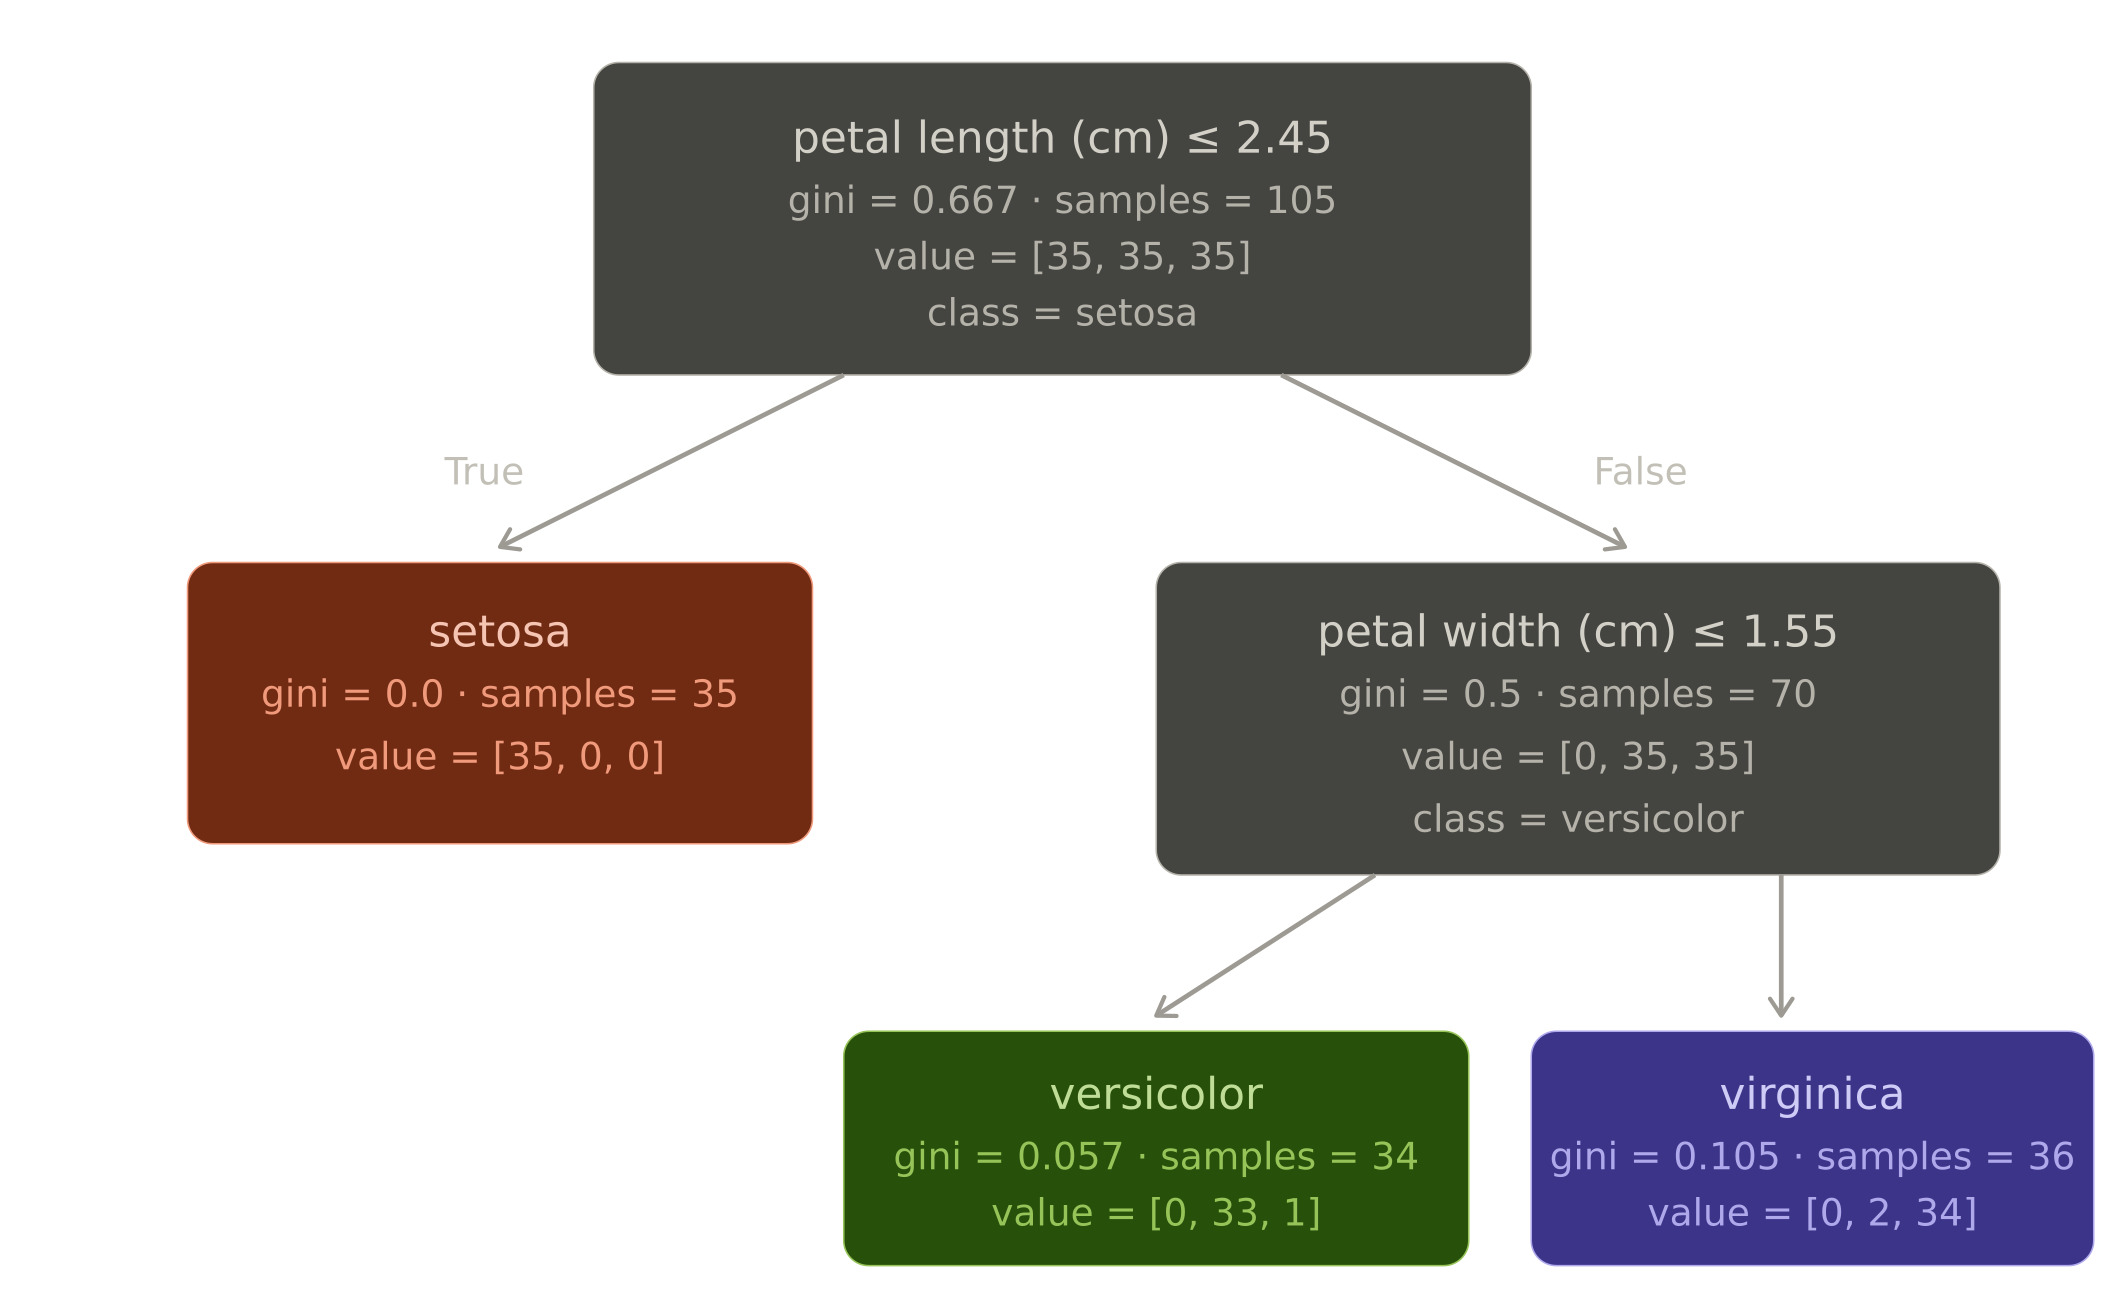
\includegraphics{iris_decision_tree.jpg}
\caption{Decision Tree Iris}
\end{figure}

    \hypertarget{domande-a-risposta-scritta}{%
\subsubsection{Domande a risposta
scritta}\label{domande-a-risposta-scritta}}

\textbf{1. Cosa rappresentano samples, value e gini in ogni nodo?}

\texttt{samples} indica il numero totale di istanze di training che
raggiungono quel nodo. \texttt{value} è un array che mostra quante di
queste istanze appartengono a ciascuna delle possibili classi di fiori.
\texttt{gini} misura l'indice di impurità del nodo: vale 0 quando tutti
i campioni appartengono a una sola classe e cresce quanto più le classi
sono mescolate.

\textbf{2. Perché alcuni nodi hanno gini = 0?}

Il nodo è puro, ovvero tutti i samples che cadono in quel nodo
appartengono alla stessa classe. Non è necessario effettuare ulteriori
split perché la classificazione è già certa.

\textbf{3. Descrivi il percorso di decisione per classificare un'Iris
come setosa.}

Partendo dal nodo radice, l'albero verifica la \texttt{petal\ length}.
Se la lunghezza del petalo è inferiore o uguale a 2.45 cm, l'istanza
segue il ramo di sinistra (``True'') e viene classificata come setosa.
Il nodo foglia risultante ha gini = 0, confermando che è un nodo puro.

    \hypertarget{passo-2---esperimenti-semplici}{%
\subsection{PASSO 2 - Esperimenti
semplici}\label{passo-2---esperimenti-semplici}}

\hypertarget{variare-la-profondituxe0}{%
\subsubsection{Variare la profondità}\label{variare-la-profondituxe0}}

    \hypertarget{max_depth1}{%
\paragraph{max\_depth=1}\label{max_depth1}}

    \begin{tcolorbox}[breakable, size=fbox, boxrule=1pt, pad at break*=1mm,colback=cellbackground, colframe=cellborder]
\prompt{In}{incolor}{ }{\boxspacing}
\begin{Verbatim}[commandchars=\\\{\}]
\PY{n}{tree\PYZus{}clf\PYZus{}1} \PY{o}{=} \PY{n}{DecisionTreeClassifier}\PY{p}{(}\PY{n}{max\PYZus{}depth}\PY{o}{=}\PY{l+m+mi}{1}\PY{p}{,} \PY{n}{random\PYZus{}state}\PY{o}{=}\PY{l+m+mi}{42}\PY{p}{)}
\PY{n}{tree\PYZus{}clf\PYZus{}1}\PY{o}{.}\PY{n}{fit}\PY{p}{(}\PY{n}{X\PYZus{}train}\PY{p}{,} \PY{n}{y\PYZus{}train}\PY{p}{)}
\end{Verbatim}
\end{tcolorbox}

    Si può notare che sia nel training che nel testing, l'accuracy è circa
0.67 (67\%), quindi si ha \textbf{underfitting}. Il modello è troppo
semplice: riesce a isolare correttamente solo la classe 0 (setosa) ma
fallisce nel distinguere le classi 1 e 2.

    \hypertarget{max_depth3}{%
\paragraph{max\_depth=3}\label{max_depth3}}

    \begin{tcolorbox}[breakable, size=fbox, boxrule=1pt, pad at break*=1mm,colback=cellbackground, colframe=cellborder]
\prompt{In}{incolor}{ }{\boxspacing}
\begin{Verbatim}[commandchars=\\\{\}]
\PY{n}{tree\PYZus{}clf\PYZus{}3} \PY{o}{=} \PY{n}{DecisionTreeClassifier}\PY{p}{(}\PY{n}{max\PYZus{}depth}\PY{o}{=}\PY{l+m+mi}{3}\PY{p}{,} \PY{n}{random\PYZus{}state}\PY{o}{=}\PY{l+m+mi}{42}\PY{p}{)}
\PY{n}{tree\PYZus{}clf\PYZus{}3}\PY{o}{.}\PY{n}{fit}\PY{p}{(}\PY{n}{X\PYZus{}train}\PY{p}{,} \PY{n}{y\PYZus{}train}\PY{p}{)}
\end{Verbatim}
\end{tcolorbox}

    L'accuracy è molto alta: 0.98 (98\%) nel training e 0.93 (93\%) nel
testing. Il modello risulta ben bilanciato, senza evidenti segni di
underfitting o overfitting. L'aumento della profondità permette
all'albero di creare regole sufficienti per distinguere con precisione
tutte e tre le classi.

    \hypertarget{max_depthnone}{%
\paragraph{max\_depth=None}\label{max_depthnone}}

    \begin{tcolorbox}[breakable, size=fbox, boxrule=1pt, pad at break*=1mm,colback=cellbackground, colframe=cellborder]
\prompt{In}{incolor}{ }{\boxspacing}
\begin{Verbatim}[commandchars=\\\{\}]
\PY{n}{tree\PYZus{}clf\PYZus{}none} \PY{o}{=} \PY{n}{DecisionTreeClassifier}\PY{p}{(}\PY{n}{max\PYZus{}depth}\PY{o}{=}\PY{k+kc}{None}\PY{p}{,} \PY{n}{random\PYZus{}state}\PY{o}{=}\PY{l+m+mi}{42}\PY{p}{)}
\PY{n}{tree\PYZus{}clf\PYZus{}none}\PY{o}{.}\PY{n}{fit}\PY{p}{(}\PY{n}{X\PYZus{}train}\PY{p}{,} \PY{n}{y\PYZus{}train}\PY{p}{)}
\end{Verbatim}
\end{tcolorbox}

    Nel training l'accuracy è 0.99 (99\%), ma nel testing rimane a 0.93
(93\%). Si osserva \textbf{overfitting}: il modello è diventato più
complesso senza migliorare le prestazioni su dati nuovi rispetto a
\texttt{max\_depth=3}.

    \hypertarget{gini-vs-entropy-max_depth3}{%
\subsubsection{Gini vs Entropy
(max\_depth=3)}\label{gini-vs-entropy-max_depth3}}

    \begin{tcolorbox}[breakable, size=fbox, boxrule=1pt, pad at break*=1mm,colback=cellbackground, colframe=cellborder]
\prompt{In}{incolor}{ }{\boxspacing}
\begin{Verbatim}[commandchars=\\\{\}]
\PY{n}{tree\PYZus{}clf\PYZus{}gini} \PY{o}{=} \PY{n}{DecisionTreeClassifier}\PY{p}{(}\PY{n}{max\PYZus{}depth}\PY{o}{=}\PY{l+m+mi}{3}\PY{p}{,} \PY{n}{random\PYZus{}state}\PY{o}{=}\PY{l+m+mi}{42}\PY{p}{,} \PY{n}{criterion}\PY{o}{=}\PY{l+s+s2}{\PYZdq{}}\PY{l+s+s2}{gini}\PY{l+s+s2}{\PYZdq{}}\PY{p}{)}
\PY{n}{tree\PYZus{}clf\PYZus{}gini}\PY{o}{.}\PY{n}{fit}\PY{p}{(}\PY{n}{X\PYZus{}train}\PY{p}{,} \PY{n}{y\PYZus{}train}\PY{p}{)}

\PY{n}{tree\PYZus{}clf\PYZus{}entropy} \PY{o}{=} \PY{n}{DecisionTreeClassifier}\PY{p}{(}\PY{n}{max\PYZus{}depth}\PY{o}{=}\PY{l+m+mi}{3}\PY{p}{,} \PY{n}{random\PYZus{}state}\PY{o}{=}\PY{l+m+mi}{42}\PY{p}{,} \PY{n}{criterion}\PY{o}{=}\PY{l+s+s2}{\PYZdq{}}\PY{l+s+s2}{entropy}\PY{l+s+s2}{\PYZdq{}}\PY{p}{)}
\PY{n}{tree\PYZus{}clf\PYZus{}entropy}\PY{o}{.}\PY{n}{fit}\PY{p}{(}\PY{n}{X\PYZus{}train}\PY{p}{,} \PY{n}{y\PYZus{}train}\PY{p}{)}
\end{Verbatim}
\end{tcolorbox}

    Confrontando i due criteri con \texttt{max\_depth=3}, le prestazioni
complessive sono uguali. Entrambi i modelli commettono in totale 2
errori sul training set e 3 errori sul test set, raggiungendo la stessa
accuracy. L'unica differenza è nella distribuzione degli errori tra le
classi 1 e 2. Ciò conferma che, per questo dataset, la scelta del
criterio di impurità (Gini o Entropia) non ha un impatto significativo
sulla capacità predittiva dell'albero.

    \hypertarget{uso-di-tutte-le-feature}{%
\subsubsection{Uso di tutte le feature}\label{uso-di-tutte-le-feature}}

    \begin{tcolorbox}[breakable, size=fbox, boxrule=1pt, pad at break*=1mm,colback=cellbackground, colframe=cellborder]
\prompt{In}{incolor}{ }{\boxspacing}
\begin{Verbatim}[commandchars=\\\{\}]
\PY{n}{X\PYZus{}all} \PY{o}{=} \PY{n}{iris}\PY{o}{.}\PY{n}{data}  \PY{c+c1}{\PYZsh{} tutte e 4 le feature}
\PY{n}{y\PYZus{}all} \PY{o}{=} \PY{n}{iris}\PY{o}{.}\PY{n}{target}

\PY{n}{X\PYZus{}train\PYZus{}all}\PY{p}{,} \PY{n}{X\PYZus{}test\PYZus{}all}\PY{p}{,} \PY{n}{y\PYZus{}train\PYZus{}all}\PY{p}{,} \PY{n}{y\PYZus{}test\PYZus{}all} \PY{o}{=} \PY{n}{train\PYZus{}test\PYZus{}split}\PY{p}{(}
    \PY{n}{X\PYZus{}all}\PY{p}{,} \PY{n}{y\PYZus{}all}\PY{p}{,} \PY{n}{test\PYZus{}size}\PY{o}{=}\PY{l+m+mf}{0.3}\PY{p}{,} \PY{n}{random\PYZus{}state}\PY{o}{=}\PY{l+m+mi}{42}\PY{p}{,} \PY{n}{stratify}\PY{o}{=}\PY{n}{y\PYZus{}all}\PY{p}{)}

\PY{n}{tree\PYZus{}clf\PYZus{}all} \PY{o}{=} \PY{n}{DecisionTreeClassifier}\PY{p}{(}\PY{n}{max\PYZus{}depth}\PY{o}{=}\PY{l+m+mi}{3}\PY{p}{,} \PY{n}{random\PYZus{}state}\PY{o}{=}\PY{l+m+mi}{42}\PY{p}{)}
\PY{n}{tree\PYZus{}clf\PYZus{}all}\PY{o}{.}\PY{n}{fit}\PY{p}{(}\PY{n}{X\PYZus{}train\PYZus{}all}\PY{p}{,} \PY{n}{y\PYZus{}train\PYZus{}all}\PY{p}{)}
\end{Verbatim}
\end{tcolorbox}

    \begin{tcolorbox}[breakable, size=fbox, boxrule=1pt, pad at break*=1mm,colback=cellbackground, colframe=cellborder]
\prompt{In}{incolor}{ }{\boxspacing}
\begin{Verbatim}[commandchars=\\\{\}]
\PY{n}{export\PYZus{}graphviz}\PY{p}{(}
    \PY{n}{tree\PYZus{}clf\PYZus{}all}\PY{p}{,}
    \PY{n}{out\PYZus{}file}\PY{o}{=}\PY{l+s+s2}{\PYZdq{}}\PY{l+s+s2}{iris\PYZus{}tree\PYZus{}all.dot}\PY{l+s+s2}{\PYZdq{}}\PY{p}{,}
    \PY{n}{feature\PYZus{}names}\PY{o}{=}\PY{n}{iris}\PY{o}{.}\PY{n}{feature\PYZus{}names}\PY{p}{,}
    \PY{n}{class\PYZus{}names}\PY{o}{=}\PY{n}{iris}\PY{o}{.}\PY{n}{target\PYZus{}names}\PY{p}{,}
    \PY{n}{rounded}\PY{o}{=}\PY{k+kc}{True}\PY{p}{,}
    \PY{n}{filled}\PY{o}{=}\PY{k+kc}{True}
\PY{p}{)}

\PY{n}{display}\PY{p}{(}\PY{n}{graphviz}\PY{o}{.}\PY{n}{Source}\PY{o}{.}\PY{n}{from\PYZus{}file}\PY{p}{(}\PY{l+s+s2}{\PYZdq{}}\PY{l+s+s2}{iris\PYZus{}tree\PYZus{}all.dot}\PY{l+s+s2}{\PYZdq{}}\PY{p}{)}\PY{p}{)}
\end{Verbatim}
\end{tcolorbox}

    In questo caso la performance migliora: l'accuracy sul test set passa da
0.93 (93\%) a 0.98 (98\%). L'albero è ancora interpretabile, anche
perché l'algoritmo ha effettuato una feature selection automatica,
utilizzando solamente le misure dei petali e non quelle dei sepali.


    % Add a bibliography block to the postdoc
    
    
    
\end{document}
